% Compile from this directory: pdflatex Assignment_2_Jesse_Levine.tex
\documentclass[11pt,letterpaper]{article}

\usepackage[T1]{fontenc}
\usepackage{lmodern}
\usepackage[margin=0.85in]{geometry}
\usepackage{amsmath,amssymb}
\usepackage{booktabs}
\usepackage{microtype}
\usepackage{float}
\usepackage[font=small,labelfont=bf,skip=5pt]{caption}
\usepackage{tikz}
\usepackage{pgfplots}
\usepackage[hidelinks]{hyperref}
\usetikzlibrary{arrows.meta,positioning,calc,shapes.geometric}
\pgfplotsset{compat=1.18}

\hypersetup{
  pdftitle={Neural Network Assignment 2},
  pdfauthor={Jesse Levine},
  pdfsubject={ELEC 5404: Neural Networks for High-Speed/High-Frequency Circuit Design}
}
\setlength{\parindent}{0pt}
\setlength{\parskip}{5pt}
\setlength{\textfloatsep}{10pt}
\setlength{\intextsep}{9pt}
\setlength{\abovedisplayskip}{8pt}
\setlength{\belowdisplayskip}{8pt}
\newcommand{\sig}{\sigma}
\newcommand{\R}{\mathbb{R}}
\newcommand{\pd}[2]{\frac{\partial #1}{\partial #2}}
\definecolor{curveblue}{RGB}{36,75,138}
\definecolor{gradred}{RGB}{190,60,40}
\pgfplotsset{
  contour plot/.style={
    axis equal image,axis lines=box,
    tick label style={font=\small},label style={font=\small},
    xlabel={$w_1$},ylabel={$w_2$},clip=true
  },
  contour/.style={black!35,line width=0.6pt,domain=0:360,samples=140,smooth},
  contour thru/.style={black!75,dashed,line width=0.8pt,domain=0:360,samples=140,smooth},
}
\tikzset{
  grad arrow/.style={-{Stealth[length=2.6mm]},gradred,line width=1.1pt},
  step arrow/.style={-{Stealth[length=2.6mm]},curveblue,line width=1.1pt},
  wpt/.style={circle,fill=curveblue,draw=white,line width=0.6pt,inner sep=1.8pt},
  lbl/.style={font=\footnotesize,inner sep=1.5pt,fill=white,fill opacity=0.85,text opacity=1},
}

\tikzset{
  neuron/.style={circle,draw,thick,minimum size=7mm,inner sep=1pt},
  input neuron/.style={neuron,minimum size=5.5mm},
  connection/.style={-{Stealth[length=2mm]},semithick},
  weight/.style={font=\small,fill=white,inner sep=1.5pt},
  bias/.style={font=\small,inner sep=1pt},
  layer/.style={font=\small\bfseries}
}

\begin{document}

\hypersetup{pageanchor=false}
\begin{titlepage}
  \centering
  \vspace*{2.24cm}
  {\Huge\bfseries Assignment \#2\par}
  \vspace{0.05cm}
  {\LARGE\itshape ELEC 5404\par}
  \vspace{1.85cm}
  {\LARGE Jesse Levine (101185127)\par}
\end{titlepage}
\pagenumbering{arabic}
\hypersetup{pageanchor=true}

\section*{Part 1: Training Numerically}

The network has one input, two sigmoid hidden neurons, and one linear output.
Train using batch-mode backpropagation with $\eta=0.1$ and no momentum. Deterimine the updated weights after one epoch.

The initial weights are
\[
\mathbf w=[v_0\;v_1\;v_2\;w_{10}\;w_{11}\;w_{20}\;w_{21}]^{T}
=[0\;\;4\;\;-1\;\;0\;\;2\;\;1\;\;0.1]^{T}.
\]

\begin{figure}[H]
\centering
\begin{minipage}[c]{0.66\linewidth}
\centering
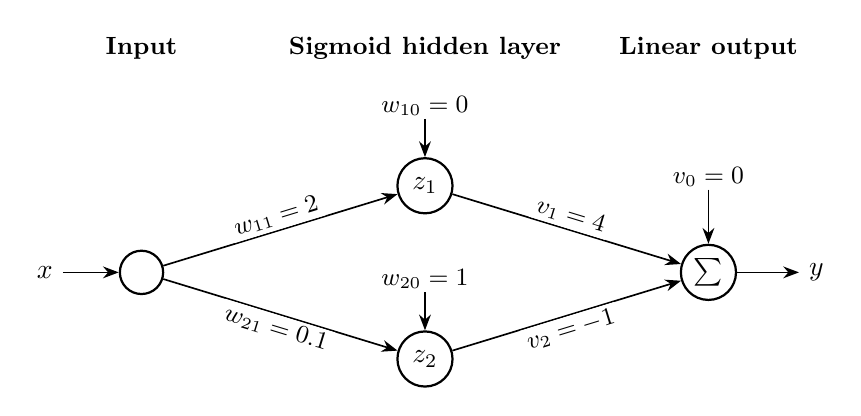
\begin{tikzpicture}
  \node[input neuron] (in) at (0,0) {};
  \node[neuron] (h1) at (3.6,1.1) {$z_1$};
  \node[neuron] (h2) at (3.6,-1.1) {$z_2$};
  \node[neuron] (out) at (7.2,0) {$\sum$};
  \node[layer] at (0,2.85) {Input};
  \node[layer] at (3.6,2.85) {Sigmoid hidden layer};
  \node[layer] at (7.2,2.85) {Linear output};
  \draw[connection] (-1,0) node[left] {$x$} -- (in);
  \draw[connection] (in) -- node[weight,above,sloped] {$w_{11}=2$} (h1);
  \draw[connection] (in) -- node[weight,below,sloped] {$w_{21}=0.1$} (h2);
  \draw[connection] (h1) -- node[weight,above,sloped] {$v_1=4$} (out);
  \draw[connection] (h2) -- node[weight,below,sloped] {$v_2=-1$} (out);
  \draw[connection] (3.6,1.95) node[bias,above] {$w_{10}=0$} -- (h1.north);
  \draw[connection] (3.6,-0.25) node[bias,above] {$w_{20}=1$} -- (h2.north);
  \draw[connection] (7.2,1.05) node[bias,above] {$v_0=0$} -- (out.north);
  \draw[connection] (out) -- (8.35,0) node[right] {$y$};
\end{tikzpicture}
\captionof{figure}{The $1$--$2$--$1$ MLP with its initial weights.}
\end{minipage}\hfill
\begin{minipage}[c]{0.3\linewidth}
\centering
\captionof{table}{Training data.}
\renewcommand{\arraystretch}{1.3}
\begin{tabular}{ccc}
\toprule
$i$ & $x_i$ & $d_i$\\
\midrule
$1$ & $0$ & $2$\\
$2$ & $1$ & $4$\\
\bottomrule
\end{tabular}
\end{minipage}
\end{figure}

The training error:
\[
E(\mathbf w)=\frac12\sum_{i=1}^{P}\bigl(y(x_i,\mathbf w)-d_i\bigr)^2 .
\]

\subsection*{(i) Forward pass of both samples}
\begin{gather*}
z_1=\sig(w_{10}+xw_{11}),\qquad z_2=\sig(w_{20}+xw_{21}),\qquad
y=v_0+v_1z_1+v_2z_2 .
\end{gather*}

\textbf{Sample 1} ($x_1=0$, $d_1=2$):
\begin{align*}
z_1&=\sig\bigl(0+(0)(2)\bigr)=\sig(0)=0.5,\\
z_2&=\sig\bigl(1+(0)(0.1)\bigr)=\sig(1)=0.7311,\\
y&=0+4(0.5)+(-1)(0.7311)=1.2689,\\
e_1&=y-d_1=1.2689-2=-0.7311.
\end{align*}

\textbf{Sample 2} ($x_2=1$, $d_2=4$):
\begin{align*}
z_1&=\sig\bigl(0+(1)(2)\bigr)=\sig(2)=0.8808,\\
z_2&=\sig\bigl(1+(1)(0.1)\bigr)=\sig(1.1)=0.7503,\\
y&=0+4(0.8808)+(-1)(0.7503)=2.7729,\\
e_2&=y-d_2=2.7729-4=-1.2271.
\end{align*}

\subsection*{(ii) Training error}

\[
E=\frac12\left(e_1^2+e_2^2\right)
=\frac12\left((-0.7311)^2+(-1.2271)^2\right)
\quad\Longrightarrow\quad \boxed{E=1.0201}.
\]

\subsection*{(iii) Derivatives w.r.t each weight}

Since $E_i=\tfrac12e_i^2$ with $e_i=y_i-d_i$, each per-sample derivative is
$\partial E_i/\partial w=e_i\,\partial y_i/\partial w$.

Therefore:
$\partial y/\partial w$ for every weight.

\textbf{Output layer.} From $y=v_0+v_1z_1+v_2z_2$,
\[
\pd{y}{v_0}=1,\qquad \pd{y}{v_1}=z_1,\qquad \pd{y}{v_2}=z_2 .
\]

\textbf{Hidden layer.} With $\gamma_1=w_{11}x+w_{10}$, I have
$\partial\gamma_1/\partial w_{11}=x$ and $\partial\gamma_1/\partial w_{10}=1$,
and the classic sigmoid derivative being $\sig'(\gamma)=z(1-z)$. Then applying chain rule,
\begin{align*}
\pd{y}{w_{11}}&=\pd{y}{z_1}\pd{z_1}{\gamma_1}\pd{\gamma_1}{w_{11}}
=v_1\,z_1(1-z_1)\,x,
&\pd{y}{w_{10}}&=v_1\,z_1(1-z_1)(1),\\[3pt]
\pd{y}{w_{21}}&=\pd{y}{z_2}\pd{z_2}{\gamma_2}\pd{\gamma_2}{w_{21}}
=v_2\,z_2(1-z_2)\,x,
&\pd{y}{w_{20}}&=v_2\,z_2(1-z_2)(1).
\end{align*}
Multiplying each by $e$ gives the per-sample error derivatives in
Table~\ref{tab:formulas}.

\begin{table}[H]
\centering
\caption{Per-sample error derivatives.}
\label{tab:formulas}
\renewcommand{\arraystretch}{1.35}
\begin{tabular}{ll}
\toprule
Weight & $\partial E_i/\partial w$\\
\midrule
$v_0$    & $e$\\
$v_1$    & $e\,z_1$\\
$v_2$    & $e\,z_2$\\
$w_{10}$ & $e\,v_1\,z_1(1-z_1)$\\
$w_{11}$ & $e\,v_1\,z_1(1-z_1)\,x$\\
$w_{20}$ & $e\,v_2\,z_2(1-z_2)$\\
$w_{21}$ & $e\,v_2\,z_2(1-z_2)\,x$\\
\bottomrule
\end{tabular}
\end{table}

\textbf{Sample 1} ($x_1=0$, $e_1=-0.7311$, $z_1=0.5$, $z_2=0.7311$):
\begin{align*}
\partial E_1/\partial v_0&=e_1=-0.7311,\\
\partial E_1/\partial v_1&=e_1z_1=(-0.7311)(0.5)=-0.3655,\\
\partial E_1/\partial v_2&=e_1z_2=(-0.7311)(0.7311)=-0.5344,\\
\partial E_1/\partial w_{10}&=e_1v_1z_1(1-z_1)=(-0.7311)(4)(0.5)(0.5)=-0.7311,\\
\partial E_1/\partial w_{11}&=e_1v_1z_1(1-z_1)\,x_1=(-0.7311)(0)=0,\\
\partial E_1/\partial w_{20}&=e_1v_2z_2(1-z_2)=(-0.7311)(-1)(0.7311)(0.2689)=0.1437,\\
\partial E_1/\partial w_{21}&=e_1v_2z_2(1-z_2)\,x_1=(0.1437)(0)=0.
\end{align*}

\textbf{Sample 2} ($x_2=1$, $e_2=-1.2271$, $z_1=0.8808$, $z_2=0.7503$):
\begin{align*}
\partial E_2/\partial v_0&=e_2=-1.2271,\\
\partial E_2/\partial v_1&=e_2z_1=(-1.2271)(0.8808)=-1.0808,\\
\partial E_2/\partial v_2&=e_2z_2=(-1.2271)(0.7503)=-0.9206,\\
\partial E_2/\partial w_{10}&=e_2v_1z_1(1-z_1)=(-1.2271)(4)(0.8808)(0.1192)=-0.5153,\\
\partial E_2/\partial w_{11}&=e_2v_1z_1(1-z_1)\,x_2=(-0.5153)(1)=-0.5153,\\
\partial E_2/\partial w_{20}&=e_2v_2z_2(1-z_2)=(-1.2271)(-1)(0.7503)(0.2497)=0.2299,\\
\partial E_2/\partial w_{21}&=e_2v_2z_2(1-z_2)\,x_2=(0.2299)(1)=0.2299.
\end{align*}

\subsection*{(iv) Sum derivatives of both samples and update}
\[
w_{\text{new}}=w_{\text{old}}-\eta\,\pd{E}{w},\qquad \eta=0.1 .
\]

\begin{table}[H]
\centering
\caption{Batch gradient and updated weights after one epoch.}
\renewcommand{\arraystretch}{1.3}
\begin{tabular}{lrrrr}
\toprule
Weight & Sample 1 & Sample 2 & $\partial E/\partial w$ & $w_{\text{new}}$\\
\midrule
$v_0$    & $-0.7311$ & $-1.2271$ & $-1.9581$ & $0.1958$\\
$v_1$    & $-0.3655$ & $-1.0808$ & $-1.4463$ & $4.1446$\\
$v_2$    & $-0.5344$ & $-0.9206$ & $-1.4551$ & $-0.8545$\\
$w_{10}$ & $-0.7311$ & $-0.5153$ & $-1.2464$ & $0.1246$\\
$w_{11}$ & $0$       & $-0.5153$ & $-0.5153$ & $2.0515$\\
$w_{20}$ & $0.1437$  & $0.2299$  & $0.3737$  & $0.9626$\\
$w_{21}$ & $0$       & $0.2299$  & $0.2299$  & $0.0770$\\
\bottomrule
\end{tabular}
\end{table}

The updated weights at the end of the first epoch are therefore
\[
\boxed{\mathbf w_{\text{new}}
=[v_0\;v_1\;v_2\;w_{10}\;w_{11}\;w_{20}\;w_{21}]^{T}
=[0.1958\;\;4.1446\;\;-0.8545\;\;0.1246\;\;2.0515\;\;0.9626\;\;0.0770]^{T}.}
\]

\clearpage
\section*{Part 2: Training by Graphical Illustration}

Let the training error and initial weights be
\[
E(\mathbf w)=w_1^2-2w_1+1+2\left(w_2^2-4w_2+4\right),\qquad
\mathbf w(0)=[0.5\;\;1]^{T}.
\]

\subsection*{(a) Batch-mode backpropagation with a contour plot}

I begin by completing the square in each bracket:
\[
E(\mathbf w)=\left(w_1^2-2w_1+1\right)+2\left(w_2^2-4w_2+4\right)
=(w_1-1)^2+2(w_2-2)^2 .
\]
Both terms are non-negative, so $E\ge0$, with $E=0$ only at the minimum
$\mathbf w^*=[1\;\;2]^{T}$.

\textbf{Contours.} Setting $E$ equal to a constant $c$ gives
\[
c=(w_1-1)^2+2(w_2-2)^2 .
\]
I then find where this contour crosses the lines through the centre. On the
horizontal line $w_2=2$,
\[
c=(w_1-1)^2\quad\Longrightarrow\quad w_1=1\pm\sqrt c ,
\]
and on the vertical line $w_1=1$,
\[
c=2(w_2-2)^2\quad\Longrightarrow\quad w_2=2\pm\sqrt{c/2}.
\]
Each contour is therefore an ellipse centred at $(1,2)$, with half-width
$\sqrt c$ along $w_1$ and half-height $\sqrt{c/2}$ along $w_2$.

\textbf{Initial point.} At $\mathbf w(0)$,
\[
E(\mathbf w(0))=(0.5-1)^2+2(1-2)^2=0.25+2=2.25 ,
\]
so the $E=2.25$ contour passes through $\mathbf w(0)$. Its points follow
from choosing $w_1$ and solving
$w_2=2\pm\sqrt{\bigl(2.25-(w_1-1)^2\bigr)/2}$:

\begin{table}[H]
\centering
\caption{Points on the $E=2.25$ contour.}
\renewcommand{\arraystretch}{1.25}
\begin{tabular}{lrrrrrrr}
\toprule
$w_1$ & $-0.5$ & $0$ & $0.5$ & $1$ & $1.5$ & $2$ & $2.5$\\
\midrule
$w_2$ (top)    & $2$ & $2.79$ & $3$ & $3.06$ & $3$ & $2.79$ & $2$\\
$w_2$ (bottom) & $2$ & $1.21$ & $1$ & $0.94$ & $1$ & $1.21$ & $2$\\
\bottomrule
\end{tabular}
\end{table}

\subsubsection*{Epoch 1}

\textbf{Gradient.} Differentiating the expanded error
$E=w_1^2-2w_1+1+2w_2^2-8w_2+8$ with respect to each weight gives
\[
\pd{E}{w_1}=2w_1-2,\qquad \pd{E}{w_2}=4w_2-8 .
\]
At $\mathbf w(0)=[0.5\;\;1]^{T}$,
\[
\pd{E}{w_1}=2(0.5)-2=-1,\qquad \pd{E}{w_2}=4(1)-8=-4
\quad\Longrightarrow\quad \nabla E=[-1\;\;-4]^{T}.
\]

\textbf{Direction.} With zero momentum, the backpropagation direction is
the negative gradient:
\[
\mathbf h=-\nabla E=[1\;\;4]^{T}.
\]

\textbf{Line minimization.} Starting at $\mathbf w(0)$, each point along
$\mathbf h$ is
\[
\mathbf w=\mathbf w(0)+\eta\,\mathbf h=[0.5\;\;1]^{T}+\eta\,[1\;\;4]^{T}
\quad\Longrightarrow\quad w_1=0.5+\eta,\qquad w_2=1+4\eta .
\]
Evaluating $E$ at trial step sizes shows that it decreases and then rises
again, with the minimum near $\eta\approx0.25$:

\begin{table}[H]
\centering
\caption{Trial step sizes along $\mathbf h$ in epoch 1.}
\renewcommand{\arraystretch}{1.2}
\begin{tabular}{rrrr}
\toprule
$\eta$ & $w_1$ & $w_2$ & $E$\\
\midrule
$0$    & $0.5$  & $1$   & $2.25$\\
$0.1$  & $0.6$  & $1.4$ & $0.88$\\
$0.2$  & $0.7$  & $1.8$ & $0.17$\\
$\mathbf{0.25}$ & $\mathbf{0.75}$ & $\mathbf{2}$ & $\mathbf{0.0625}$\\
$0.3$  & $0.8$  & $2.2$ & $0.12$\\
$0.4$  & $0.9$  & $2.6$ & $0.73$\\
$0.5$  & $1$    & $3$   & $2$\\
\bottomrule
\end{tabular}
\end{table}

To find the exact minimum, I substitute the line into $E$:
\[
E(\eta)=(0.5+\eta-1)^2+2(4\eta-1)^2=33\eta^2-17\eta+2.25 .
\]
Setting the derivative to zero,
\[
\frac{dE}{d\eta}=66\eta-17=0
\quad\Longrightarrow\quad \eta=\frac{17}{66}=0.2576 .
\]
The new weights at the end of epoch 1 are therefore
\begin{align*}
w_1&=0.5+0.2576=0.7576,\\
w_2&=1+4(0.2576)=2.0303,
\end{align*}
\[
\boxed{\mathbf w(1)=[0.7576\;\;2.0303]^{T}},\qquad
E=(0.7576-1)^2+2(2.0303-2)^2=0.0606 .
\]

\subsubsection*{Epoch 2}

\textbf{Gradient and direction.} At $\mathbf w(1)$,
\[
\pd{E}{w_1}=2(0.7576)-2=-0.4848,\qquad
\pd{E}{w_2}=4(2.0303)-8=0.1212 ,
\]
\[
\nabla E=[-0.4848\;\;0.1212]^{T},\qquad
\mathbf h=-\nabla E=[0.4848\;\;-0.1212]^{T}.
\]

\textbf{Line minimization.} Each point along the new direction is
\[
\mathbf w=[0.7576\;\;2.0303]^{T}+\eta\,[0.4848\;\;-0.1212]^{T}
\quad\Longrightarrow\quad
w_1=0.7576+0.4848\eta,\qquad w_2=2.0303-0.1212\eta .
\]

\begin{table}[H]
\centering
\caption{Trial step sizes along $\mathbf h$ in epoch 2.}
\renewcommand{\arraystretch}{1.2}
\begin{tabular}{rrrr}
\toprule
$\eta$ & $w_1$ & $w_2$ & $E$\\
\midrule
$0$   & $0.7576$ & $2.0303$ & $0.0606$\\
$0.2$ & $0.8546$ & $2.0061$ & $0.0212$\\
$0.4$ & $0.9515$ & $1.9818$ & $0.0030$\\
$\mathbf{0.5}$ & $\mathbf{1}$ & $\mathbf{1.9697}$ & $\mathbf{0.0018}$\\
$0.6$ & $1.0485$ & $1.9576$ & $0.0059$\\
$0.8$ & $1.1454$ & $1.9333$ & $0.0300$\\
\bottomrule
\end{tabular}
\end{table}

The minimum lies between $\eta=0.4$ and $\eta=0.5$. Substituting the line into $E$,
\[
E(\eta)=(0.4848\eta-0.2424)^2+2(0.0303-0.1212\eta)^2
=0.2644\eta^2-0.2497\eta+0.0606 ,
\]
\[
\frac{dE}{d\eta}=0.5288\eta-0.2497=0
\quad\Longrightarrow\quad \eta=\frac{0.2497}{0.5288}=0.4722 .
\]
The weights at the end of epoch 2 are therefore
\[
\boxed{\mathbf w(2)=[0.9865\;\;1.9731]^{T}},\qquad E=0.00163 .
\]

\textbf{Contour plot.} Figure~\ref{fig:sd} shows the contours, the initial
point, the gradient and search direction in each epoch, and the location of
$\mathbf w$ after each epoch. Each line search ends where the search line is
tangent to a contour. The two search directions are perpendicular, since
$[1\;\;4]\cdot[0.4848\;\;-0.1212]=0$. The path therefore zig-zags, and after two
epochs $\mathbf w(2)$ is close to, but not at, the minimum $\mathbf w^*=[1\;\;2]^{T}$.

\begin{figure}[H]
\centering
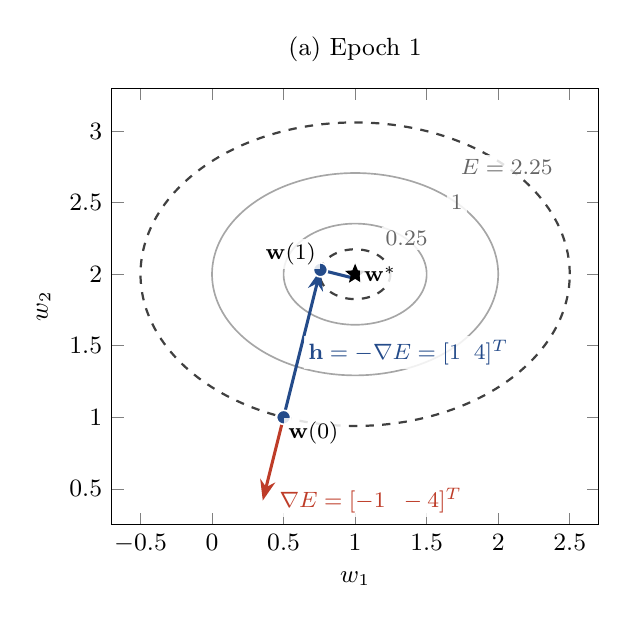
\begin{tikzpicture}
\begin{axis}[contour plot,width=0.64\linewidth,height=0.64\linewidth,
  xmin=-0.7,xmax=2.7,ymin=0.25,ymax=3.3,
  xtick={-0.5,0,0.5,1,1.5,2,2.5},ytick={0.5,1,1.5,2,2.5,3},
  title={\small (a) Epoch 1}]
  % contours
  \addplot[contour] ({1+1.0*cos(x)},{2+0.70711*sin(x)});
  \addplot[contour] ({1+0.5*cos(x)},{2+0.35355*sin(x)});
  \addplot[contour thru] ({1+1.5*cos(x)},{2+1.06066*sin(x)});
  \addplot[contour thru] ({1+0.24618*cos(x)},{2+0.17408*sin(x)});
  \node[lbl,text=black!60] at (2.06,2.75) {$E=2.25$};
  \node[lbl,text=black!60] at (1.71,2.50) {$1$};
  \node[lbl,text=black!60] at (1.36,2.25) {$0.25$};
  % epoch 1
  \draw[grad arrow] (0.5,1) -- (0.3545,0.418)
    node[lbl,right,xshift=4pt,text=gradred] {$\nabla E=[-1\;\;-4]^T$};
  \draw[step arrow] (0.5,1) -- (0.7576,2.0303);
  \node[lbl,right,text=curveblue] at (0.64,1.45) {$\mathbf h=-\nabla E=[1\;\;4]^T$};
  \draw[curveblue,line width=1.1pt] (0.7576,2.0303) -- (0.9865,1.9731);
  % points
  \node[wpt] at (0.5,1) {};
  \node[lbl,below right] at (0.5,1) {$\mathbf w(0)$};
  \node[wpt] at (0.7576,2.0303) {};
  \node[lbl,above left] at (0.7576,2.0303) {$\mathbf w(1)$};
  \node[star,star points=5,star point ratio=2.25,fill=black,inner sep=1.2pt] at (1,2) {};
  \node[lbl,anchor=west] at (1.03,2.0) {$\mathbf w^*$};
\end{axis}
\end{tikzpicture}

\vspace{4mm}
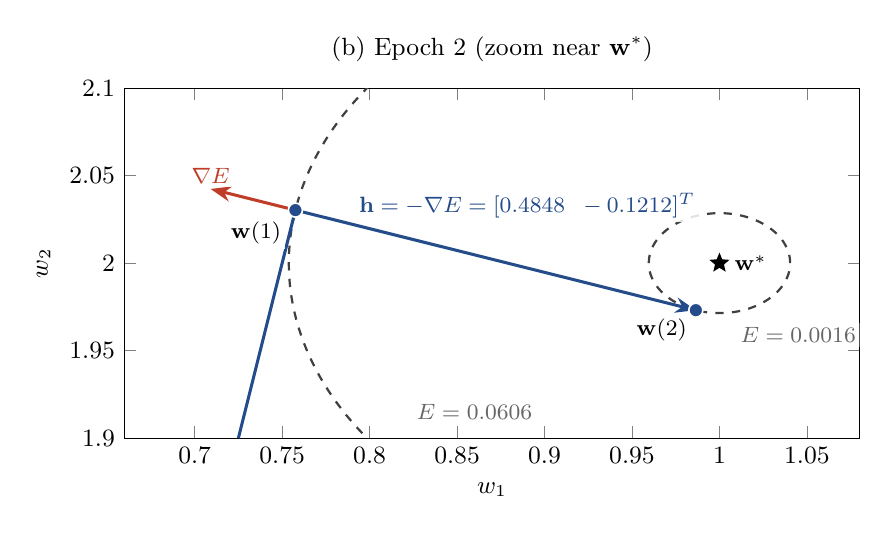
\begin{tikzpicture}
\begin{axis}[contour plot,width=0.9\linewidth,height=0.5\linewidth,
  xmin=0.66,xmax=1.08,ymin=1.90,ymax=2.10,
  xtick={0.7,0.75,0.8,0.85,0.9,0.95,1.0,1.05},ytick={1.9,1.95,2,2.05,2.1},
  xticklabel style={/pgf/number format/fixed,/pgf/number format/precision=2},
  yticklabel style={/pgf/number format/fixed,/pgf/number format/precision=2},
  title={\small (b) Epoch 2 (zoom near $\mathbf w^*$)}]
  % contours through w(1) and w(2)
  \addplot[contour thru] ({1+0.24618*cos(x)},{2+0.17408*sin(x)});
  \addplot[contour thru] ({1+0.040404*cos(x)},{2+0.028570*sin(x)});
  \node[lbl,text=black!60] at (0.86,1.915) {$E=0.0606$};
  \node[lbl,text=black!60,anchor=north] at (1.045,1.966) {$E=0.0016$};
  % incoming epoch-1 line
  \draw[curveblue,line width=1.1pt] (0.7250,1.90) -- (0.7576,2.0303);
  % right-angle mark at w(1)
  \draw[black!70,line width=0.5pt]
    ($(0.7576,2.0303)+(-0.0029,-0.01164)$) --
    ($(0.7576,2.0303)+(-0.0029,-0.01164)+(0.01164,-0.0029)$) --
    ($(0.7576,2.0303)+(0.01164,-0.0029)$);
  % epoch 2
  \draw[grad arrow] (0.7576,2.0303) -- (0.7091,2.0424)
    node[lbl,above,text=gradred] {$\nabla E$};
  \draw[step arrow] (0.7576,2.0303) -- (0.9865,1.9731);
  \node[lbl,text=curveblue,anchor=south] at (0.89,2.023) {$\mathbf h=-\nabla E=[0.4848\;\;-0.1212]^T$};
  % points
  \node[wpt] at (0.7576,2.0303) {};
  \node[lbl,anchor=north east] at (0.752,2.026) {$\mathbf w(1)$};
  \node[wpt] at (0.9865,1.9731) {};
  \node[lbl,anchor=north east] at (0.984,1.971) {$\mathbf w(2)$};
  \node[star,star points=5,star point ratio=2.25,fill=black,inner sep=1.2pt] at (1,2) {};
  \node[lbl,anchor=west] at (1.006,2.0) {$\mathbf w^*$};
\end{axis}
\end{tikzpicture}
\caption{Batch-mode backpropagation with line minimization. Dashed contours
pass through $\mathbf w(0)$, $\mathbf w(1)$ and $\mathbf w(2)$. Red arrows show
$\nabla E$ and blue arrows show $\mathbf h=-\nabla E$ (directions only, not to
scale). Panel (b) enlarges the region around $\mathbf w^*$ to show epoch 2.}
\label{fig:sd}
\end{figure}

\subsection*{(b) Conjugate gradient method}

\textbf{1. Number of epochs.} Two epochs are needed, because there are two
weights. $E$ is a quadratic function of the $n=2$ weights, and with exact line
minimization, the conjugate gradient method reaches the minimum of an $n$-weight
quadratic in at most $n$ epochs. This is confirmed below, where $E=0$ at the end
of epoch 2.

\textbf{2. Epoch 1.} With no previous direction, the first conjugate gradient
epoch is identical to epoch 1 of part (a):
\[
\nabla E(\mathbf w(0))=[-1\;\;-4]^{T},\qquad
\mathbf h_0=-\nabla E=[1\;\;4]^{T},\qquad \eta=0.2576 ,
\]
\[
\mathbf w(1)=[0.7576\;\;2.0303]^{T},\qquad E=0.0606 .
\]

\textbf{3. Negative gradient in epoch 2.} Epoch 2 begins as in part (a):
\[
\pd{E}{w_1}=2(0.7576)-2=-0.4848,\qquad
\pd{E}{w_2}=4(2.0303)-8=0.1212 ,
\]
\[
\nabla E(\mathbf w(1))=[-0.4848\;\;0.1212]^{T}
\quad\Longrightarrow\quad
-\nabla E(\mathbf w(1))=[0.4848\;\;-0.1212]^{T}.
\]

\textbf{4. Conjugate gradient direction.} The new direction combines the
negative gradient with the previous direction:
\[
\mathbf h_1=-\nabla E(\mathbf w(1))+\gamma\,\mathbf h_0 .
\]
Using the Fletcher--Reeves formula,
\[
\gamma=\frac{\lvert\nabla E(\mathbf w(1))\rvert^2}{\lvert\nabla E(\mathbf w(0))\rvert^2}
=\frac{(-0.4848)^2+(0.1212)^2}{(-1)^2+(-4)^2}
=\frac{0.2497}{17}=0.0147 .
\]
Therefore,
\[
\mathbf h_1=[0.4848\;\;-0.1212]^{T}+0.0147\,[1\;\;4]^{T}
=[0.4848\;\;-0.1212]^{T}+[0.0147\;\;0.0588]^{T}
=[0.4995\;\;-0.0624]^{T}.
\]

\textbf{5. Line minimization and the location of $\mathbf w$ after epoch 2.}
Each point along $\mathbf h_1$ is
\[
\mathbf w=[0.7576\;\;2.0303]^{T}+\eta\,[0.4995\;\;-0.0624]^{T}
\quad\Longrightarrow\quad
w_1=0.7576+0.4995\eta,\qquad w_2=2.0303-0.0624\eta .
\]

\begin{table}[H]
\centering
\caption{Trial step sizes along the conjugate direction $\mathbf h_1$ in epoch 2.}
\renewcommand{\arraystretch}{1.2}
\begin{tabular}{rrrr}
\toprule
$\eta$ & $w_1$ & $w_2$ & $E$\\
\midrule
$0$   & $0.7576$ & $2.0303$ & $0.0606$\\
$0.2$ & $0.8575$ & $2.0178$ & $0.0209$\\
$0.4$ & $0.9574$ & $2.0053$ & $0.0019$\\
$\mathbf{0.5}$ & $\mathbf{1.0073}$ & $\mathbf{1.9991}$ & $\mathbf{0.0001}$\\
$0.6$ & $1.0573$ & $1.9928$ & $0.0034$\\
$0.8$ & $1.1572$ & $1.9803$ & $0.0255$\\
\bottomrule
\end{tabular}
\end{table}

The minimum lies near $\eta=0.5$, where $E$ is already almost zero.
Substituting the line into $E$,
\[
E(\eta)=(0.4995\eta-0.2424)^2+2(0.0303-0.0624\eta)^2
=0.25729\eta^2-0.24972\eta+0.06061 ,
\]
\[
\frac{dE}{d\eta}=0.51458\eta-0.24972=0
\quad\Longrightarrow\quad \eta=\frac{0.24972}{0.51458}=0.4853 .
\]
The weights at the end of epoch 2 are therefore
\begin{align*}
w_1&=0.7576+0.4995(0.4853)=0.7576+0.2424=1.0000,\\
w_2&=2.0303-0.0624(0.4853)=2.0303-0.0303=2.0000,
\end{align*}
\[
\boxed{\mathbf w(2)=[1\;\;2]^{T}=\mathbf w^*},\qquad
E=(1-1)^2+2(2-2)^2=0 .
\]
The training error reaches zero after two epochs, as stated in item 1.

\textbf{Contour plot.} Figure~\ref{fig:cg} shows the conjugate gradient
training. Epoch 1 is the same as in Figure~\ref{fig:sd}. In epoch 2, adding
$\gamma\mathbf h_0$ to $-\nabla E$ tilts the direction from $[4\;\;-1]$ to
$[0.4995\;\;-0.0624]\propto[8\;\;-1]$. This is exactly the direction from
$\mathbf w(1)$ to the minimum, $\mathbf w^*-\mathbf w(1)=[0.2424\;\;-0.0303]^{T}$.
The two search directions are conjugate rather than perpendicular:
$\mathbf h_0^{T}\,\mathrm{diag}(2,4)\,\mathbf h_1=2(1)(0.4995)+4(4)(-0.0624)\approx0$.

\begin{figure}[H]
\centering
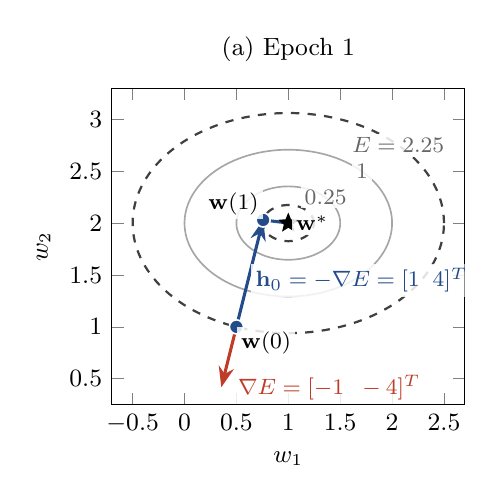
\begin{tikzpicture}
\begin{axis}[contour plot,width=0.5\linewidth,height=0.5\linewidth,
  xmin=-0.7,xmax=2.7,ymin=0.25,ymax=3.3,
  xtick={-0.5,0,0.5,1,1.5,2,2.5},ytick={0.5,1,1.5,2,2.5,3},
  title={\small (a) Epoch 1}]
  \addplot[contour] ({1+1.0*cos(x)},{2+0.70711*sin(x)});
  \addplot[contour] ({1+0.5*cos(x)},{2+0.35355*sin(x)});
  \addplot[contour thru] ({1+1.5*cos(x)},{2+1.06066*sin(x)});
  \addplot[contour thru] ({1+0.24618*cos(x)},{2+0.17408*sin(x)});
  \node[lbl,text=black!60] at (2.06,2.75) {$E=2.25$};
  \node[lbl,text=black!60] at (1.71,2.50) {$1$};
  \node[lbl,text=black!60] at (1.36,2.25) {$0.25$};
  \draw[grad arrow] (0.5,1) -- (0.3545,0.418)
    node[lbl,right,xshift=4pt,text=gradred] {$\nabla E=[-1\;\;-4]^T$};
  \draw[step arrow] (0.5,1) -- (0.7576,2.0303);
  \node[lbl,right,text=curveblue] at (0.64,1.45) {$\mathbf h_0=-\nabla E=[1\;\;4]^T$};
  \draw[curveblue,line width=1.1pt] (0.7576,2.0303) -- (1,2);
  \node[wpt] at (0.5,1) {};
  \node[lbl,below right] at (0.5,1) {$\mathbf w(0)$};
  \node[wpt] at (0.7576,2.0303) {};
  \node[lbl,above left] at (0.7576,2.0303) {$\mathbf w(1)$};
  \node[star,star points=5,star point ratio=2.25,fill=black,inner sep=1.2pt] at (1,2) {};
  \node[lbl,anchor=west] at (1.03,2.0) {$\mathbf w^*$};
\end{axis}
\end{tikzpicture}

\vspace{2mm}
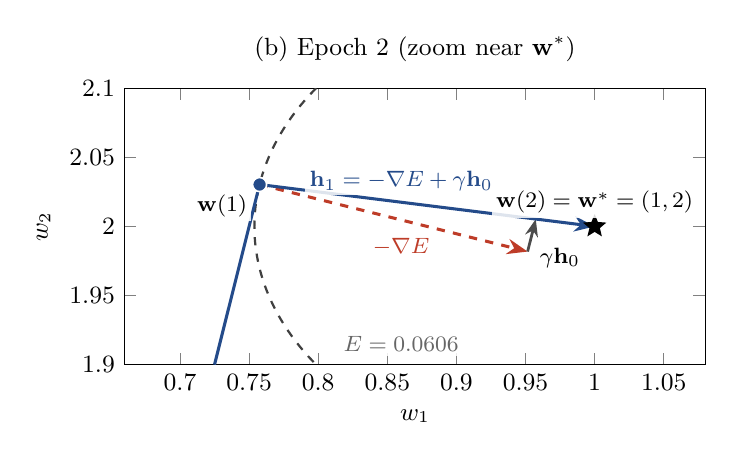
\begin{tikzpicture}
\begin{axis}[contour plot,width=0.82\linewidth,height=0.42\linewidth,
  xmin=0.66,xmax=1.08,ymin=1.90,ymax=2.10,
  xtick={0.7,0.75,0.8,0.85,0.9,0.95,1.0,1.05},ytick={1.9,1.95,2,2.05,2.1},
  xticklabel style={/pgf/number format/fixed,/pgf/number format/precision=2},
  yticklabel style={/pgf/number format/fixed,/pgf/number format/precision=2},
  title={\small (b) Epoch 2 (zoom near $\mathbf w^*$)}]
  \addplot[contour thru] ({1+0.24618*cos(x)},{2+0.17408*sin(x)});
  \node[lbl,text=black!60] at (0.86,1.915) {$E=0.0606$};
  % incoming epoch-1 line
  \draw[curveblue,line width=1.1pt] (0.7250,1.90) -- (0.7576,2.0303);
  % -grad E, then + gamma h0 (both scaled by 0.4), resultant h1 points at w*
  \draw[grad arrow,dashed] (0.7576,2.0303) -- (0.9515,1.9818);
  \node[lbl,text=gradred,anchor=north] at (0.86,1.995) {$-\nabla E$};
  \draw[-{Stealth[length=2.2mm]},black!70,line width=1pt] (0.9515,1.9818) -- (0.9574,2.0053);
  \node[lbl,anchor=north west] at (0.957,1.988) {$\gamma\mathbf h_0$};
  \draw[step arrow] (0.7576,2.0303) -- (1,2);
  \node[lbl,text=curveblue,anchor=south] at (0.86,2.022) {$\mathbf h_1=-\nabla E+\gamma\mathbf h_0$};
  \node[wpt] at (0.7576,2.0303) {};
  \node[lbl,anchor=north east] at (0.752,2.026) {$\mathbf w(1)$};
  \node[star,star points=5,star point ratio=2.25,fill=black,inner sep=1.4pt] at (1,2) {};
  \node[lbl,anchor=south] at (1.0,2.006) {$\mathbf w(2)=\mathbf w^*=(1,2)$};
\end{axis}
\end{tikzpicture}
\caption{Conjugate gradient training with line minimization. Epoch 1 is
identical to part (a). In epoch 2, the dashed red arrow is the negative gradient,
the grey arrow is $\gamma\mathbf h_0$ (vectors scaled for visibility), and their sum
$\mathbf h_1$ leads directly to the minimum, so $E=0$ after two epochs.}
\label{fig:cg}
\end{figure}

\end{document}
